% Copyright (C) 2018 Liu Yifan, Zhao Tianyu 
% Permission is granted to copy, distribute and/or modify this document
% under the terms of the GNU Free Documentation License, Version 1.3
% or any later version published by the Free Software Foundation;
% with no Invariant Sections, no FrontCover Texts, and no BackCover Texts.
% A copy of the license is included in the section entitled "GNU
% Free Documentation License".
%%%%%%%%%%%%%%%%重要的事情现在前面,第一次编译点左上角选 Compiler(编译器)为XeLaTeX%%%%%%%%%%%%
\documentclass[zihao=-4,a4paper]{ctexart}

% 论文基本配置,加载宏包、数学命令等全局配置
% Copyright (C) 2018 Liu Yifan, Zhao Tianyu 
% Permission is granted to copy, distribute and/or modify this document
% under the terms of the GNU Free Documentation License, Version 1.3
% or any later version published by the Free Software Foundation;
% with no Invariant Sections, no FrontCover Texts, and no BackCover Texts.
% A copy of the license is included in the section entitled "GNU
% Free Documentation License".
\usepackage{ctex}
\setCJKmainfont[AutoFakeBold=2, ItalicFont={simsun.ttc}]{simsun.ttc}
\setmainfont{Times New Roman} 
\usepackage{fontspec}
\usepackage{amsmath}
\usepackage{amssymb}
\usepackage{hyperref} 
\usepackage{amsthm} 
\usepackage{mathtools} 
\usepackage{mathrsfs}
\usepackage{fancyhdr}
\usepackage{enumerate}
\usepackage{metalogo}
% \usepackage{mathscr}
\numberwithin{equation}{section}
\newtheorem{definition}{定义}[section]
\newtheorem{example}{例}[section]
\newtheorem{theorem}{定理}[section]
\newtheorem*{maintheorem}{主要定理}
\newtheorem{question}{问题}
\newtheorem{lemma}[theorem]{引理}
\newtheorem{remark}[theorem]{备注}
\newtheorem{corollary}[theorem]{推论}
\newtheorem{proposition}[theorem]{命题}
%\songti
% \newtheorem{algorithm}
\ctexset{section={format={\zihao{3}\bfseries},
			name = {第,章},beforeskip=0.5ex plus 20pt,afterskip=10pt}}
\ctexset{subsection={format={\zihao{4}\bfseries },
				beforeskip=0.75ex,afterskip=0.95ex}}
\ctexset{subsubsection={format={\zihao{-4}\bfseries },
				beforeskip=0.75ex,afterskip=0.95ex}}

\usepackage{caption}
\captionsetup{font={small},labelsep=space}
\numberwithin{figure}{section}
\renewcommand{\proofname}{\zihao{-4}  \bfseries 证明}
\usepackage{geometry}
\geometry{top=2.5cm,bottom=2.5cm,left=3cm,right=2.5cm,headsep=0.5cm}
%\setmainfont{Times New Roman}
\ctexset{abstractname={\zihao{3}   摘\hspace*{2em} 要}}
%\ctexset{abstract={beforskip={20pt}
		%	     afterskip=10pt}}
\ctexset{bibname={\centerline{ \zihao{3}  参\hspace*{0.5em}考\hspace*{0.5em}文\hspace*{0.5em}献}}}
%\ctexset{section ={name = {第,章},beforeskip=20pt,afterskip=10pt}}
\usepackage{setspace}

\usepackage{listings} 
\usepackage{natbib}
\setcitestyle{numbers,square,comma}
%\setlength{\bibspacing}{\baselineskip}

\newcommand{\upcite}[1]{\textsuperscript{\cite{#1}}}

\usepackage{titletoc}
\titlecontents{section}[0pt]{\addvspace{2pt}\filright}
{\contentspush{\thecontentslabel\ }}
{}{\titlerule*[8pt]{.}\contentspage}
%%%%commented%%%%
%\usepackage{enumitem}
%\setenumerate{fullwidth,itemindent=\parindent,listparindent=\parindent,itemsep=0ex,partopsep=0pt,parsep=0ex}

\usepackage{graphicx}
\usepackage{caption}
\usepackage{subfigure}
%%%%%%%%%%%%%5
\usepackage{enumerate}
\usepackage{minted}
%%%%%%%%%%%%%
\usepackage{pdfpages}
\usepackage{afterpage}
\allowdisplaybreaks[1]


\newcommand{\h}{\tilde{h}}
\renewcommand{\k}{\kappa}
\renewcommand{\b}{\beta}
\renewcommand{\t}{\theta}
\newcommand{\la}{\lambda}
\newcommand{\La}{\Lambda}
\newcommand{\kk}{\tilde{\kappa}}
\renewcommand{\L}{\mathscr{L}}
\newcommand{\A}{\mathscr{A}}
\newcommand{\F}{\mathbf{F}}
\newcommand{\p}{\mathbf{p}}
%%%%%%%%%%%%%%%%%fanfan%%%%%%

\newcommand{\blank}[1]{\hspace*{#1}}
\newcommand{\sectionend}{\ifodd\value{page}\afterpage{\null\newpage}\else\fi\newpage\vspace*{0pt}}
\usepackage{dutchcal}
%%%%%%%%%%%%%%%%%%%%%%%%%%%%%%%

\pagestyle{fancy}
\lhead{}
\rhead{}
\chead{\zihao{-5} 论文题目}
\cfoot{\zihao{-5} \thepage}
\renewcommand{\headrulewidth}{0.4pt}
\renewcommand{\footrulewidth}{0pt}



\title{\zihao{2} \bfseries  论文题目}
\author{}
\date{}



% 表格中支持跨行
%\usepackage{multirow}

% 跨页表格
%\usepackage{longtable}

% 固定宽度的表格
%\usepackage{tabularx}

% 表格中的反斜线
%\usepackage{diagbox}

% 确定浮动对象的位置,可以使用 H,强制将浮动对象放到这里(可能效果很差)
%\usepackage{float}

% 浮动图形控制宏包。
% 允许上一个 section 的浮动图形出现在下一个 section 的开始部分
% 该宏包提供处理浮动对象的 \FloatBarrier 命令,使所有未处
% 理的浮动图形立即被处理。这三个宏包仅供参考,未必使用:
% \usepackage[below]{placeins}
% \usepackage{floatflt} % 图文混排用宏包
% \usepackage{rotating} % 图形和表格的控制旋转

% 定理类环境宏包
%\usepackage[amsmath,thmmarks,hyperref]{ntheorem}


% 数学命令
%% Adapted for use with thuthesis.
% Original code is at https://github.com/goodfeli/dlbook_notation/blob/master/math_commands.tex

%%%%% NEW MATH DEFINITIONS %%%%%

\newcommand\ceil[1]{\lceil #1 \rceil}
\newcommand\floor[1]{\lfloor #1 \rfloor}


% Vectors
\newcommand\Vector[1]{\symbf{#1}}

\newcommand\0{{\Vector{0}}}
\newcommand\vzero{{\Vector{0}}}
\newcommand\1{{\Vector{1}}}
\newcommand\vone{{\Vector{1}}}

\newcommand\va{{\Vector{a}}}
\newcommand\vb{{\Vector{b}}}
\newcommand\vc{{\Vector{c}}}
\newcommand\vd{{\Vector{d}}}
\newcommand\ve{{\Vector{e}}}
\newcommand\vf{{\Vector{f}}}
\newcommand\vg{{\Vector{g}}}
\newcommand\vh{{\Vector{h}}}
\newcommand\vi{{\Vector{i}}}
\newcommand\vj{{\Vector{j}}}
\newcommand\vk{{\Vector{k}}}
\newcommand\vl{{\Vector{l}}}
\newcommand\vm{{\Vector{m}}}
\newcommand\vn{{\Vector{n}}}
\newcommand\vo{{\Vector{o}}}
\newcommand\vp{{\Vector{p}}}
\newcommand\vq{{\Vector{q}}}
\newcommand\vr{{\Vector{r}}}
\newcommand\vs{{\Vector{s}}}
\newcommand\vt{{\Vector{t}}}
\newcommand\vu{{\Vector{u}}}
\newcommand\vv{{\Vector{v}}}
\newcommand\vw{{\Vector{w}}}
\newcommand\vx{{\Vector{x}}}
\newcommand\vy{{\Vector{y}}}
\newcommand\vz{{\Vector{z}}}

\newcommand\valpha{{\Vector{\alpha}}}
\newcommand\vbeta{{\Vector{\beta}}}
\newcommand\vgamma{{\Vector{\gamma}}}
\newcommand\vdelta{{\Vector{\delta}}}
\newcommand\vepsilon{{\Vector{\epsilon}}}
\newcommand\vtheta{{\Vector{\theta}}}
\newcommand\viota{{\Vector{\iota}}}
\newcommand\vkappa{{\Vector{\kappa}}}
\newcommand\vlambda{{\Vector{\lambda}}}
\newcommand\vmu{{\Vector{\mu}}}
\newcommand\vnu{{\Vector{\nu}}}
\newcommand\vxi{{\Vector{\xi}}}
\newcommand\vpi{{\Vector{\pi}}}
\newcommand\vrho{{\Vector{\rho}}}
\newcommand\vsigma{{\Vector{\sigma}}}
\newcommand\vtau{{\Vector{\tau}}}
\newcommand\vupsilon{{\Vector{\upsilon}}}
\newcommand\vphi{{\Vector{\phi}}}
\newcommand\vchi{{\Vector{\chi}}}
\newcommand\vpsi{{\Vector{\psi}}}
\newcommand\vomega{{\Vector{\omega}}}


% Matrix
\newcommand\MATRIX[1]{\symbf{#1}}

\newcommand\mA{{\MATRIX{A}}}
\newcommand\mB{{\MATRIX{B}}}
\newcommand\mC{{\MATRIX{C}}}
\newcommand\mD{{\MATRIX{D}}}
\newcommand\mE{{\MATRIX{E}}}
\newcommand\mF{{\MATRIX{F}}}
\newcommand\mG{{\MATRIX{G}}}
\newcommand\mH{{\MATRIX{H}}}
\newcommand\mI{{\MATRIX{I}}}
\newcommand\mJ{{\MATRIX{J}}}
\newcommand\mK{{\MATRIX{K}}}
\newcommand\mL{{\MATRIX{L}}}
\newcommand\mM{{\MATRIX{M}}}
\newcommand\mN{{\MATRIX{N}}}
\newcommand\mO{{\MATRIX{O}}}
\newcommand\mP{{\MATRIX{P}}}
\newcommand\mQ{{\MATRIX{Q}}}
\newcommand\mR{{\MATRIX{R}}}
\newcommand\mS{{\MATRIX{S}}}
\newcommand\mT{{\MATRIX{T}}}
\newcommand\mU{{\MATRIX{U}}}
\newcommand\mV{{\MATRIX{V}}}
\newcommand\mW{{\MATRIX{W}}}
\newcommand\mX{{\MATRIX{X}}}
\newcommand\mY{{\MATRIX{Y}}}
\newcommand\mZ{{\MATRIX{Z}}}

\newcommand\mGamma{{\MATRIX{\Gamma}}}
\newcommand\mDelta{{\MATRIX{\Delta}}}
\newcommand\mTheta{{\MATRIX{\Theta}}}
\newcommand\mLambda{{\MATRIX{\Lambda}}}
\newcommand\mXi{{\MATRIX{\Xi}}}
\newcommand\mPi{{\MATRIX{\Pi}}}
\newcommand\mSigma{{\MATRIX{\Sigma}}}
\newcommand\mUpsilon{{\MATRIX{\Upsilon}}}
\newcommand\mPhi{{\MATRIX{\Phi}}}
\newcommand\mPsi{{\MATRIX{\Psi}}}
\newcommand\mOmega{{\MATRIX{\Omega}}}


% Tensor
\newcommand\tens[1]{\symbfsf{#1}}
\newcommand\tA{{\tens{A}}}
\newcommand\tB{{\tens{B}}}
\newcommand\tC{{\tens{C}}}
\newcommand\tD{{\tens{D}}}
\newcommand\tE{{\tens{E}}}
\newcommand\tF{{\tens{F}}}
\newcommand\tG{{\tens{G}}}
\newcommand\tH{{\tens{H}}}
\newcommand\tI{{\tens{I}}}
\newcommand\tJ{{\tens{J}}}
\newcommand\tK{{\tens{K}}}
\newcommand\tL{{\tens{L}}}
\newcommand\tM{{\tens{M}}}
\newcommand\tN{{\tens{N}}}
\newcommand\tO{{\tens{O}}}
\newcommand\tP{{\tens{P}}}
\newcommand\tQ{{\tens{Q}}}
\newcommand\tR{{\tens{R}}}
\newcommand\tS{{\tens{S}}}
\newcommand\tT{{\tens{T}}}
\newcommand\tU{{\tens{U}}}
\newcommand\tV{{\tens{V}}}
\newcommand\tW{{\tens{W}}}
\newcommand\tX{{\tens{X}}}
\newcommand\tY{{\tens{Y}}}
\newcommand\tZ{{\tens{Z}}}


% Graph
\newcommand\gA{{\mathcal{A}}}
\newcommand\gB{{\mathcal{B}}}
\newcommand\gC{{\mathcal{C}}}
\newcommand\gD{{\mathcal{D}}}
\newcommand\gE{{\mathcal{E}}}
\newcommand\gF{{\mathcal{F}}}
\newcommand\gG{{\mathcal{G}}}
\newcommand\gH{{\mathcal{H}}}
\newcommand\gI{{\mathcal{I}}}
\newcommand\gJ{{\mathcal{J}}}
\newcommand\gK{{\mathcal{K}}}
\newcommand\gL{{\mathcal{L}}}
\newcommand\gM{{\mathcal{M}}}
\newcommand\gN{{\mathcal{N}}}
\newcommand\gO{{\mathcal{O}}}
\newcommand\gP{{\mathcal{P}}}
\newcommand\gQ{{\mathcal{Q}}}
\newcommand\gR{{\mathcal{R}}}
\newcommand\gS{{\mathcal{S}}}
\newcommand\gT{{\mathcal{T}}}
\newcommand\gU{{\mathcal{U}}}
\newcommand\gV{{\mathcal{V}}}
\newcommand\gW{{\mathcal{W}}}
\newcommand\gX{{\mathcal{X}}}
\newcommand\gY{{\mathcal{Y}}}
\newcommand\gZ{{\mathcal{Z}}}


% Sets
\newcommand\sA{{\mathbb{A}}}
\newcommand\sB{{\mathbb{B}}}
\newcommand\sC{{\mathbb{C}}}
\newcommand\sD{{\mathbb{D}}}
% Don't use a set called E, because this would be the same as our symbol
% for expectation.
\newcommand\sF{{\mathbb{F}}}
\newcommand\sG{{\mathbb{G}}}
\newcommand\sH{{\mathbb{H}}}
\newcommand\sI{{\mathbb{I}}}
\newcommand\sJ{{\mathbb{J}}}
\newcommand\sK{{\mathbb{K}}}
\newcommand\sL{{\mathbb{L}}}
\newcommand\sM{{\mathbb{M}}}
\newcommand\sN{{\mathbb{N}}}
\newcommand\sO{{\mathbb{O}}}
\newcommand\sP{{\mathbb{P}}}
\newcommand\sQ{{\mathbb{Q}}}
\newcommand\sR{{\mathbb{R}}}
\newcommand\sS{{\mathbb{S}}}
\newcommand\sT{{\mathbb{T}}}
\newcommand\sU{{\mathbb{U}}}
\newcommand\sV{{\mathbb{V}}}
\newcommand\sW{{\mathbb{W}}}
\newcommand\sX{{\mathbb{X}}}
\newcommand\sY{{\mathbb{Y}}}
\newcommand\sZ{{\mathbb{Z}}}


% Random variables
\newcommand\RandomVariable[1]{\symit{#1}}

\newcommand\rA{{\RandomVariable{A}}}
\newcommand\rB{{\RandomVariable{B}}}
\newcommand\rC{{\RandomVariable{C}}}
\newcommand\rD{{\RandomVariable{D}}}
\newcommand\rE{{\RandomVariable{E}}}
\newcommand\rF{{\RandomVariable{F}}}
\newcommand\rG{{\RandomVariable{G}}}
\newcommand\rH{{\RandomVariable{H}}}
\newcommand\rI{{\RandomVariable{I}}}
\newcommand\rJ{{\RandomVariable{J}}}
\newcommand\rK{{\RandomVariable{K}}}
\newcommand\rL{{\RandomVariable{L}}}
\newcommand\rM{{\RandomVariable{M}}}
\newcommand\rN{{\RandomVariable{N}}}
\newcommand\rO{{\RandomVariable{O}}}
\newcommand\rP{{\RandomVariable{P}}}
\newcommand\rQ{{\RandomVariable{Q}}}
\newcommand\rR{{\RandomVariable{R}}}
\newcommand\rS{{\RandomVariable{S}}}
\newcommand\rT{{\RandomVariable{T}}}
\newcommand\rU{{\RandomVariable{U}}}
\newcommand\rV{{\RandomVariable{V}}}
\newcommand\rW{{\RandomVariable{W}}}
\newcommand\rX{{\RandomVariable{X}}}
\newcommand\rY{{\RandomVariable{Y}}}
\newcommand\rZ{{\RandomVariable{Z}}}

% Random vectors
\newcommand\RandomVector[1]{\symbf{#1}}

\newcommand\rvA{{\RandomVector{A}}}
\newcommand\rvB{{\RandomVector{B}}}
\newcommand\rvC{{\RandomVector{C}}}
\newcommand\rvD{{\RandomVector{D}}}
\newcommand\rvE{{\RandomVector{E}}}
\newcommand\rvF{{\RandomVector{F}}}
\newcommand\rvG{{\RandomVector{G}}}
\newcommand\rvH{{\RandomVector{H}}}
\newcommand\rvI{{\RandomVector{I}}}
\newcommand\rvJ{{\RandomVector{J}}}
\newcommand\rvK{{\RandomVector{K}}}
\newcommand\rvL{{\RandomVector{L}}}
\newcommand\rvM{{\RandomVector{M}}}
\newcommand\rvN{{\RandomVector{N}}}
\newcommand\rvO{{\RandomVector{O}}}
\newcommand\rvP{{\RandomVector{P}}}
\newcommand\rvQ{{\RandomVector{Q}}}
\newcommand\rvR{{\RandomVector{R}}}
\newcommand\rvS{{\RandomVector{S}}}
\newcommand\rvT{{\RandomVector{T}}}
\newcommand\rvU{{\RandomVector{U}}}
\newcommand\rvV{{\RandomVector{V}}}
\newcommand\rvW{{\RandomVector{W}}}
\newcommand\rvX{{\RandomVector{X}}}
\newcommand\rvY{{\RandomVector{Y}}}
\newcommand\rvZ{{\RandomVector{Z}}}

\newcommand\laplace{\mathrm{Laplace}} % Laplace distribution

\newcommand\E{\mathbb{E}}
\newcommand\Ls{\mathcal{L}}
\newcommand\R{\mathbb{R}}
\newcommand\emp{\tilde{p}}
\newcommand\lr{\alpha}
\newcommand\reg{\lambda}
\newcommand\rect{\mathrm{rectifier}}
\newcommand\softmax{\mathrm{softmax}}
\newcommand\sigmoid{\sigma}
\newcommand\softplus{\zeta}
\newcommand\KL{D_{\mathrm{KL}}}
\newcommand\Var{\mathrm{Var}}
\newcommand\standarderror{\mathrm{SE}}
\newcommand\Cov{\mathrm{Cov}}
% Wolfram Mathworld says $L^2$ is for function spaces and $\ell^2$ is for vectors
% But then they seem to use $L^2$ for vectors throughout the site, and so does
% wikipedia.
\newcommand\normlzero{L^0}
\newcommand\normlone{L^1}
\newcommand\normltwo{L^2}
\newcommand\normlp{L^p}
\newcommand\normmax{L^\infty}

\DeclareMathOperator*{\argmax}{arg\,max}
\DeclareMathOperator*{\argmin}{arg\,min}

\DeclareMathOperator{\sign}{sign}
\DeclareMathOperator{\Tr}{Tr}
\let\ab\allowbreak


% 定义自己常用的东西
% \def\myname{薛瑞尼}




% hyperref 宏包在最后调用
\usepackage{hyperref}
% algorithms
\usepackage[ruled,vlined]{algorithm2e}
\renewcommand{\algorithmcfname}{算法}

\usepackage{booktabs}
% \usepackage{xcolor}
% 据说加了一行这个查重就不会乱码了
% \usepackage{ccmap}
\begin{document}
        %  \begin{center}
        %   求解多右端线性方程组的一种改进共轭梯度算法研究\\
        %   %{\bfseries \zihao{2} !如果不多加这一行字复制进Word会乱码,导致不能查重!}
        %  \end{center}

	\includepdfmerge{cover.pdf,1-2}
	
	\thispagestyle{plain}
	\pagenumbering{Roman}
	\linespread{1.35}
	\begin{abstract}
	\zihao{-4}{
	目前在众多学科领域都需要求解多右端项线性方程组,本文
	..
	
	..
	
	..
	到校正矩阵Frobenius范数的最小值。最后通过Julia程序对其进行对比数值试验。
	\\
	\\
	{\bfseries  关键词: 关键词1,关键词2} }
	\end{abstract}


	

	
	\newpage
	\thispagestyle{plain}
	\renewcommand\abstractname{ABSTRACT}
	
	\begin{abstract}
	\zihao{-4}{
	At present, it is necessary to solve multi-right-end linear equations in many disciplines. This paper 
	..
	
	..
	algorithms can converge to the minimum of the Frobenius norm value.
	\\
	\\
	{\bf Keywords: 
KW1,KW2}     }
	\end{abstract}
	
	\newpage
	\thispagestyle{plain}
	\renewcommand\contentsname{\centerline{\zihao{3}    目\hspace*{2em}录}}

	\tableofcontents
% 
	
	\newpage
	
	%\maketitle
	\thispagestyle{fancy}
	\vspace*{-20pt}
	\begin{center}
	\zihao{3} \bfseries  论文题目
	\vspace*{20pt}
	\end{center}
	
	\pagenumbering{arabic}
	
% \mainmatter
% Copyright (C) 2018 Liu Yifan, Zhao Tianyu 
% Permission is granted to copy, distribute and/or modify this document
% under the terms of the GNU Free Documentation License, Version 1.3
% or any later version published by the Free Software Foundation;
% with no Invariant Sections, no FrontCover Texts, and no BackCover Texts.
% A copy of the license is included in the section entitled "GNU
% Free Documentation License".

\section{为什么要做这个模板}\label{ch:intr}


因为使用Microsoft 
Word写学术论文是一件非常自我摧残的事情,要花费大量的时间去学习Word排版,
弄不好还要花费别人大量的时间帮忙排自己的论文,还要搭上人情,请人家吃饭什么的,
在别人心中留下一个小小的印记:“切,连排个版都不会!”

关键是用Word写学术论文本来就是一件十分不靠谱的事情,而且完全有更简单,更专业的解决方法 —— {\LaTeX} !

既然你下载了这个模板,而且有看文档的好习惯,那么恭喜你吞下了那颗红色小药丸!

Welcome to the real world!

其实下面的内容你都没有必要看的,就是例行的啰嗦啰嗦,你可以直接跳到
第\ref{ch:install}章。(看到了吧,pdf文档里面可以有超链接,你Word弄个超链接
出来费劲死了。)

\subsection{模板说明}
\label{sec:fastguide}

\subsubsection{模板特性}
\label{sec:features}

这个模板是大连海事大学数学系本科生毕业论文\LaTeX{}模版,中文解决方案是\XeLaTeX和CTex。

此版本由数学系应数2014级Zhao Tianyu和LiuYifan的论文模板改进完成。

由2016级Esther适配Overleaf。

\textbf{年代久远,请留意后续学校论文格式变动}


\textbf{重要的事情现在前面,第一次编译点左上角选 Compiler 为 \XeLaTeX}
配置在Dmusetup.tex中 

建议完整看完本教程,没时间也要看第四章, 下面是一部分重点和建议
\begin{enumerate}
    \item 配置在Dmusetup.tex中 
    \item /fig /photo /text 等文件夹即字面意思
    \item 知网查重提交pdf 会乱码 可转成word再进行查重, Linux 下转换word命令行为: 
    \begin{lstlisting}
pandoc ./main.tex --bibliography refs.bib  -o output.doc
#带reference 不推荐
pandoc ./main.tex   -o output.doc 
#推荐不带reference 并需要根据报错删除致谢一类的章节
  \end{lstlisting}
  \item 各位置的题目 设定没有同步,须设定多处,e.g., 页眉
  \item 有不懂的问题,先看overleaf的document\href{https://www.overleaf.com/learn}{"点此"},和stackoverflow自行搜索. 若还有问题到本项目主页"点击此处"开issues反馈.
  \item 引用分清楚\cite{hart_initializing_2012}和\upcite{hart_initializing_2012} 的区别
\end{enumerate}

 





 \sectionend
% Copyright (C) 2018 Liu Yifan, Zhibo Xiao and Vital Delmas Mabonzo
% Copyright (C) 2018 Liu Yifan, Zhao Tianyu 
% Permission is granted to copy, distribute and/or modify this document
% under the terms of the GNU Free Documentation License, Version 1.3
% or any later version published by the Free Software Foundation;
% with no Invariant Sections, no FrontCover Texts, and no BackCover Texts.
% A copy of the license is included in the section entitled "GNU
% Free Documentation License".

\section{模板的安装使用}\label{ch:install}

\textbf{使用平台编译请看视频教程,e.g.,\href{https://www.youtube.com/playlist?list=PLnC5h3PY-znyDQKn3knfXfekZLgWyL7QW}{Minimal examples of LaTeX with overleaf (v2)}}.

下面的文字教程适用于本地编译

原本内容已经被注释掉,想看请到源码ch2.tex中看,选中下面文字部分  ctrl+/  解除注释 再编译

% \subsection{安装 \TeX 系统}
% \subsubsection{Windows}
% 考虑到Windows系统用户大多数使用CTex(基于MiKTeX),这里只说明CTex的安装方法。
% \begin{enumerate}
% \item 下载CTex v2.9完整版,\url{http://www.ctex.org/CTeXDownload};
% \item 按照第\ref{sect:compile}节的方法编译你的论文即可。
% \end{enumerate}

% \subsubsection{Mac OSX}

% 完整安装MacTeX套装即可。

% \subsubsection{Linux}

% 完整安装TeXLive最新版即可。




% \subsection{编译你的论文}\label{sect:compile}

% 论文的中英文封面和原创性声明需要使用Word编辑,并且在每页之后添加一个空白页(Ctrl+Enter),然后将前六页保存成pdf文件——cover.pdf。

% 之后在body文件夹用文本编辑器打开各个源文件进行编辑。

% \subsubsection{文本编辑器}

% 不要使用CTex套装中预制了WinEdt编辑器,否则后果自负。
% 由于WinEdt使用GBK编码。插入参考文献时需要配合另外的软件
% 使用,大多数软件默认的编码都是UTF8,所以不推荐WinEdt,我们推荐使用
% TexStudio、Vim+LaTexSuite等支持UTF8编码的专用LaTeX编辑器进行编辑。
% 也可以使用Sublime Text 2、Notepad++等其他纯文本编辑器。

% 文本编辑器推荐列表(依照推荐顺序排序):

% \begin{itemize}
% \item IDE组
% \begin{enumerate}
% 	\item TeXstudio
% 	\item Texmaker
% 	\item TeXnicCenter
% \end{enumerate}
% \item{纯文本编辑器组}
% \begin{enumerate}
% \item Vim+LaTeXSuite (神器)
% \item Sublime Text 2
% \end{enumerate}
% \end{itemize}


% \subsubsection{快捷编译}

% 如果确保使用的\LaTeX 命令没有错误,可以使用模板附带的批处理命令进行编译。
% \subsubsection{Windows下编译}

% 双击 \texttt{run.bat}文件进行编辑。

% \subsubsection{Mac OSX和Linux下编译}

% 在你最喜欢的bash下面运行\texttt{make} 编译。
% 或者运行\texttt{sh run.sh}编译。

% \subsubsection{使用命令行编译}

% 这种方式在所有系统下都可以进行。打开命令行工具,进入模板所在文件夹,按照下面顺序依次输入:
% \begin{verbatim}
% xelatex dmuthesis
% bibtex dmuthesis
% xelatex dmuthesis
% xelatex dmuthesis
% \end{verbatim}
% 为了生成参考文献和书签以及交叉引用,所有的\LaTeX 文件都需要编译4次,\XeLaTeX 
% 文件也不例外。

 \sectionend
% % Copyright (C) 2018 Liu Yifan, Zhao Tianyu 
% Permission is granted to copy, distribute and/or modify this document
% under the terms of the GNU Free Documentation License, Version 1.3
% or any later version published by the Free Software Foundation;
% with no Invariant Sections, no FrontCover Texts, and no BackCover Texts.
% A copy of the license is included in the section entitled "GNU
% Free Documentation License".
\section{如何解决一些现实问题}
原本内容已经被注释掉,想看请到源码ch3.tex中看,选中下面文字部分  ctrl+/  解除注释 再编译
% \subsection{如何解决查新的问题}

% 由于查新仅仅是通过字符串匹配的问题,所以只要把文中的字符复制到Word里面即可,不用考虑格式的问题。下面提供几种将pdf文件转成word格式的方法,所有内容来自善用佳软上的文章\textbf{PDF转换word格式的方法总结}(\url{http://xbeta.info/pdf2word.htm})。

% \subsubsection{推荐的PDF转换word方案}

% PDFtoWord.com(\url{http://www.pdftoword.com/}) 号称是目前最为精准的pdf to word文件转换器,出自著名的PDF解决方案供应商NitroPDF。PDFtoWord.com是在线应用,完全免费,使用方便:
% \begin{enumerate}
% \item 访问pdftoword.com
% \item 上传pdf
% \item 输入接收邮箱
% \item 进入邮箱:查收转换后的word文档。
% \end{enumerate}
% 推荐这个网站的原因是这个网站对中文的支持非常好,而且Pdftoword 在排版方面确实有独到之处,特别介绍一个细节,Pdftoword 转换后的文档仍以段落为单位,没有很多的换行符,而以前大多转换器都是以行为单位,以致末尾有很多的换行符,你复制粘贴时会有许多麻烦。


% \subsection{如果忘了\LaTeX 命令怎么写该怎么办?}

% \url{http://www.biwako.shiga-u.ac.jp/sensei/kumazawa/texindex3.html#formula}

% \subsection{避免常见的\LaTeX 错误}

% \begin{itemize}
% \item Journal of Machine Learning Research 对于论文投稿论文的一些要求 (\url{http://jmlr.csail.mit.edu/format/format.html})
% \item 有关中文本地化的内容
% \item LATEX for Complete Novices \url{www.dickimaw-books.com/latex/novices/} 
% \end{itemize}

% \begin{description}

% \item[破折号] 在句子中使用\raisebox{0.5mm}{---}破折号\raisebox{0.5mm}{---}达到插入效果的时候要特别小心。
% 破折号要长,并且在破折号之前和之后的都不应该有空格。
% 并且中文的破折号与英文的破折号高度不一样,所以\LaTeX 原始输入为:
% \begin{verbatim}
% 在句子中使用\raisebox{0.5mm}{---}破折号\raisebox{0.5mm}{---}达到插入效果的时候要特别小心。
% \end{verbatim}
% \item[小写名称及缩写名称]文中出现的领域名称,算法名称,方法名称等都应该使用小写字母,比如:cognitive science, reinforcement learning, principal components analysis。
% 当涉及到组织名,比如Cognitive Science Department,或者涉及专有名词,比如Markov decision processes, Gaussian densities, Bayes' rule时才需要大写。

% 后文反复提到的缩写名称应该在文中第一次提及时给出完整的英文全程和缩写,比如隐狄利克雷分配(Latent Dirichlet Allocation, LDA)。
% 这样,在后文就可以使用LDA指代隐狄利克雷分配了。
% \item[拉丁缩写]首先,文中不鼓励使用拉丁缩写。建议使用中文替代,``i.e.'' 替换为“即”,``e.g.''替换为“例如”。如果你实在是要用拉丁缩写,一定要使用正确,即,在每个字母后面都要有一个半角句号。
% \item[公式编号]当且仅当后文要引用这个公式的时候才为这个公式编号。
% \item[参考文献标引]参考文献标引在文中并不是名词。下面的语句是不对的:
% \begin{verbatim}
% 利用[34]的方法,我们如何如何
% \end{verbatim}
% 正确的句式为:
% \begin{verbatim}
% 利用Smith在文献[23]提出的方法,我们如何如何
% \end{verbatim}
% 或者:
% \begin{verbatim}
% 利用非线性降维方法[34],我们如何如何。
% \end{verbatim}
% \item[不要使用utilize这个词]
% \item[不要在一个段落后马上加入子段落]在两个段落之间应该有链接句子,不允许出现下面的情况:
% \begin{verbatim}
% 5. 实验结果

% 5.1 退化实验结果
% \end{verbatim}
% 正确的格式为:
% \begin{verbatim}
% 5. 实验结果

% 在这一章,我们首先描述了 blah, blah, blah

% 5.1 退化实验结果
% \end{verbatim}
% \item[float环境位置]All text references to a table should be by a number, not
% by an introductory phrase such as ‘in the following table’.”
% \item[unbreakable space] 
% \begin{verbatim}
% Figure~\ref{fig:single} shows some shapes.
% \end{verbatim}
% 效果为:Figure shows some shapes.
% \item[math mode] 当输入变量的时候,一定要在数学模式输入,比如 $x,y,z$,而不是x,y,z.
% \item[数学公式引用] \verb|\eqref{label} = (\ref{label})|
% \item[eqnarray] Don’t use the \texttt{eqnarray} or \texttt{eqnarray*} environments. They’re obsolete
% \item[数学模式中插入文字]
% \begin{align*} 
% y &= 2x + 2\\
% \intertext{Using the distributive law:中文也可以}
% &= 2(x+1)
% \end{align*}
% \begin{verbatim}
% \begin{align*} 
% y &= 2x + 2\\
% \intertext{Using the distributive law:中文也可以}
% &= 2(x+1)
% \end{align*}
% \end{verbatim}
% \item[数学字体] \verb \mathcal{text}  只对大写字母起作用
% \begin{table}[htbp]
% \centering
% \begin{tabular}{cc}
% \hline 
% Example Input & Corresponding Output \\ 
% \hline
% \verb$\mathrm{xyz}$& $\mathrm{xyz}$ \\ 
% \verb$\mathsf{xyz}$& $\mathsf{xyz}$  \\ 
% \verb$\mathtt{xyz}$& $\mathtt{xyz}$   \\ 
% \verb$\mathit{xyz}$& $\mathit{xyz}$   \\ 
% \verb$\mathbf{xyz}$& $\mathbf{xyz}$   \\ 
% \verb$\mathcal{OXYZ}$& $\mathcal{OXYZ}$   \\ 
% \hline 
% \end{tabular} 
% \end{table}
% 花体数学字体
% \begin{table}
% \centering
% \begin{tabular}{cc}
% \hline
% Example Input  & Example Output \\ 
% \hline
% \verb$\mathbb{A+B=C}$  & $\mathbb{A+B=C}$ \\ 
% \verb$\mathfrak{A+B=C}$  & $\mathfrak{A+B=C}$ \\ 
% \verb$\boldsymbol{A+B=C}$  & $\boldsymbol{A+B=C}$ \\ 
% \verb$\pmb{+-=}$ &    $\pmb{+-=}$\\ 
% \hline 
% \end{tabular} 
% \end{table}
% \item[希腊字母]

% \begin{table}[htbp]
% \caption{Lower Case Greek Letters}
% \label{tab:greek}
% \centering
% \begin{tabular}{llllll}
% {alpha} & $\alpha$ &
% {beta} & $\beta$ &
% {gamma} & $\gamma$ \\
% {delta} & $\delta$  &
% {epsilon} & $\epsilon$ &
% {varepsilon} & $\varepsilon$\\
% {zeta} & $\zeta$ &
% {eta} & $\eta$ &
% {theta} & $\theta$ \\
% {vartheta} & $\vartheta$ &
% {iota} & $\iota$ & 
% {kappa} & $\kappa$ \\
% {lambda} & $\lambda$ &
% {mu} & $\mu$ &
% {nu} & $\nu$ \\
% {xi} & $\xi$ &
% {pi} & $\pi$ &
% {varpi} & $\varpi$\\
% {rho} & $\rho$ &
% {varrho} & $\varrho$ &
% {sigma} & $\sigma$ \\
% {varsigma} & $\varsigma$ &
% {tau} & $\tau$ &
% {upsilon} & $\upsilon$ \\
% {phi} & $\phi$ &
% {varphi} & $\varphi$ &
% {chi} & $\chi$ \\
% {psi} & $\psi$ &
% {omega} & $\omega$ 
% \end{tabular}
% \end{table}

% \begin{table}[htbp]
% \caption{Upper Case Greek Letters}
% \label{tab:Greek}
% \centering
% \begin{tabular}{llllll}
% {Gamma} & $\Gamma$ &
% {Delta} & $\Delta$ &
% {Theta} & $\Theta$ \\
% {Lambda} & $\Lambda$ &
% {Xi} & $\Xi$ &
% {Pi} & $\Pi$ \\
% {Sigma} & $\Sigma$ &
% {Upsilon} & $\Upsilon$ &
% {Phi} & $\Phi$ \\
% {Psi} & $\Psi$ &
% {Omega} & $\Omega$
% \end{tabular}
% \end{table}


% \end{description}






 \sectionend
% Copyright (C) 2018 Liu Yifan, Zhao Tianyu 
% Permission is granted to copy, distribute and/or modify this document
% under the terms of the GNU Free Documentation License, Version 1.3
% or any later version published by the Free Software Foundation;
% with no Invariant Sections, no FrontCover Texts, and no BackCover Texts.
% A copy of the license is included in the section entitled "GNU
% Free Documentation License".
\section{如何解决一些现实问题}
原本内容已经被注释掉,想看请到源码ch3.tex中看,选中下面文字部分  ctrl+/  解除注释 再编译
% \subsection{如何解决查新的问题}

% 由于查新仅仅是通过字符串匹配的问题,所以只要把文中的字符复制到Word里面即可,不用考虑格式的问题。下面提供几种将pdf文件转成word格式的方法,所有内容来自善用佳软上的文章\textbf{PDF转换word格式的方法总结}(\url{http://xbeta.info/pdf2word.htm})。

% \subsubsection{推荐的PDF转换word方案}

% PDFtoWord.com(\url{http://www.pdftoword.com/}) 号称是目前最为精准的pdf to word文件转换器,出自著名的PDF解决方案供应商NitroPDF。PDFtoWord.com是在线应用,完全免费,使用方便:
% \begin{enumerate}
% \item 访问pdftoword.com
% \item 上传pdf
% \item 输入接收邮箱
% \item 进入邮箱:查收转换后的word文档。
% \end{enumerate}
% 推荐这个网站的原因是这个网站对中文的支持非常好,而且Pdftoword 在排版方面确实有独到之处,特别介绍一个细节,Pdftoword 转换后的文档仍以段落为单位,没有很多的换行符,而以前大多转换器都是以行为单位,以致末尾有很多的换行符,你复制粘贴时会有许多麻烦。


% \subsection{如果忘了\LaTeX 命令怎么写该怎么办?}

% \url{http://www.biwako.shiga-u.ac.jp/sensei/kumazawa/texindex3.html#formula}

% \subsection{避免常见的\LaTeX 错误}

% \begin{itemize}
% \item Journal of Machine Learning Research 对于论文投稿论文的一些要求 (\url{http://jmlr.csail.mit.edu/format/format.html})
% \item 有关中文本地化的内容
% \item LATEX for Complete Novices \url{www.dickimaw-books.com/latex/novices/} 
% \end{itemize}

% \begin{description}

% \item[破折号] 在句子中使用\raisebox{0.5mm}{---}破折号\raisebox{0.5mm}{---}达到插入效果的时候要特别小心。
% 破折号要长,并且在破折号之前和之后的都不应该有空格。
% 并且中文的破折号与英文的破折号高度不一样,所以\LaTeX 原始输入为:
% \begin{verbatim}
% 在句子中使用\raisebox{0.5mm}{---}破折号\raisebox{0.5mm}{---}达到插入效果的时候要特别小心。
% \end{verbatim}
% \item[小写名称及缩写名称]文中出现的领域名称,算法名称,方法名称等都应该使用小写字母,比如:cognitive science, reinforcement learning, principal components analysis。
% 当涉及到组织名,比如Cognitive Science Department,或者涉及专有名词,比如Markov decision processes, Gaussian densities, Bayes' rule时才需要大写。

% 后文反复提到的缩写名称应该在文中第一次提及时给出完整的英文全程和缩写,比如隐狄利克雷分配(Latent Dirichlet Allocation, LDA)。
% 这样,在后文就可以使用LDA指代隐狄利克雷分配了。
% \item[拉丁缩写]首先,文中不鼓励使用拉丁缩写。建议使用中文替代,``i.e.'' 替换为“即”,``e.g.''替换为“例如”。如果你实在是要用拉丁缩写,一定要使用正确,即,在每个字母后面都要有一个半角句号。
% \item[公式编号]当且仅当后文要引用这个公式的时候才为这个公式编号。
% \item[参考文献标引]参考文献标引在文中并不是名词。下面的语句是不对的:
% \begin{verbatim}
% 利用[34]的方法,我们如何如何
% \end{verbatim}
% 正确的句式为:
% \begin{verbatim}
% 利用Smith在文献[23]提出的方法,我们如何如何
% \end{verbatim}
% 或者:
% \begin{verbatim}
% 利用非线性降维方法[34],我们如何如何。
% \end{verbatim}
% \item[不要使用utilize这个词]
% \item[不要在一个段落后马上加入子段落]在两个段落之间应该有链接句子,不允许出现下面的情况:
% \begin{verbatim}
% 5. 实验结果

% 5.1 退化实验结果
% \end{verbatim}
% 正确的格式为:
% \begin{verbatim}
% 5. 实验结果

% 在这一章,我们首先描述了 blah, blah, blah

% 5.1 退化实验结果
% \end{verbatim}
% \item[float环境位置]All text references to a table should be by a number, not
% by an introductory phrase such as ‘in the following table’.”
% \item[unbreakable space] 
% \begin{verbatim}
% Figure~\ref{fig:single} shows some shapes.
% \end{verbatim}
% 效果为:Figure shows some shapes.
% \item[math mode] 当输入变量的时候,一定要在数学模式输入,比如 $x,y,z$,而不是x,y,z.
% \item[数学公式引用] \verb|\eqref{label} = (\ref{label})|
% \item[eqnarray] Don’t use the \texttt{eqnarray} or \texttt{eqnarray*} environments. They’re obsolete
% \item[数学模式中插入文字]
% \begin{align*} 
% y &= 2x + 2\\
% \intertext{Using the distributive law:中文也可以}
% &= 2(x+1)
% \end{align*}
% \begin{verbatim}
% \begin{align*} 
% y &= 2x + 2\\
% \intertext{Using the distributive law:中文也可以}
% &= 2(x+1)
% \end{align*}
% \end{verbatim}
% \item[数学字体] \verb \mathcal{text}  只对大写字母起作用
% \begin{table}[htbp]
% \centering
% \begin{tabular}{cc}
% \hline 
% Example Input & Corresponding Output \\ 
% \hline
% \verb$\mathrm{xyz}$& $\mathrm{xyz}$ \\ 
% \verb$\mathsf{xyz}$& $\mathsf{xyz}$  \\ 
% \verb$\mathtt{xyz}$& $\mathtt{xyz}$   \\ 
% \verb$\mathit{xyz}$& $\mathit{xyz}$   \\ 
% \verb$\mathbf{xyz}$& $\mathbf{xyz}$   \\ 
% \verb$\mathcal{OXYZ}$& $\mathcal{OXYZ}$   \\ 
% \hline 
% \end{tabular} 
% \end{table}
% 花体数学字体
% \begin{table}
% \centering
% \begin{tabular}{cc}
% \hline
% Example Input  & Example Output \\ 
% \hline
% \verb$\mathbb{A+B=C}$  & $\mathbb{A+B=C}$ \\ 
% \verb$\mathfrak{A+B=C}$  & $\mathfrak{A+B=C}$ \\ 
% \verb$\boldsymbol{A+B=C}$  & $\boldsymbol{A+B=C}$ \\ 
% \verb$\pmb{+-=}$ &    $\pmb{+-=}$\\ 
% \hline 
% \end{tabular} 
% \end{table}
% \item[希腊字母]

% \begin{table}[htbp]
% \caption{Lower Case Greek Letters}
% \label{tab:greek}
% \centering
% \begin{tabular}{llllll}
% {alpha} & $\alpha$ &
% {beta} & $\beta$ &
% {gamma} & $\gamma$ \\
% {delta} & $\delta$  &
% {epsilon} & $\epsilon$ &
% {varepsilon} & $\varepsilon$\\
% {zeta} & $\zeta$ &
% {eta} & $\eta$ &
% {theta} & $\theta$ \\
% {vartheta} & $\vartheta$ &
% {iota} & $\iota$ & 
% {kappa} & $\kappa$ \\
% {lambda} & $\lambda$ &
% {mu} & $\mu$ &
% {nu} & $\nu$ \\
% {xi} & $\xi$ &
% {pi} & $\pi$ &
% {varpi} & $\varpi$\\
% {rho} & $\rho$ &
% {varrho} & $\varrho$ &
% {sigma} & $\sigma$ \\
% {varsigma} & $\varsigma$ &
% {tau} & $\tau$ &
% {upsilon} & $\upsilon$ \\
% {phi} & $\phi$ &
% {varphi} & $\varphi$ &
% {chi} & $\chi$ \\
% {psi} & $\psi$ &
% {omega} & $\omega$ 
% \end{tabular}
% \end{table}

% \begin{table}[htbp]
% \caption{Upper Case Greek Letters}
% \label{tab:Greek}
% \centering
% \begin{tabular}{llllll}
% {Gamma} & $\Gamma$ &
% {Delta} & $\Delta$ &
% {Theta} & $\Theta$ \\
% {Lambda} & $\Lambda$ &
% {Xi} & $\Xi$ &
% {Pi} & $\Pi$ \\
% {Sigma} & $\Sigma$ &
% {Upsilon} & $\Upsilon$ &
% {Phi} & $\Phi$ \\
% {Psi} & $\Psi$ &
% {Omega} & $\Omega$
% \end{tabular}
% \end{table}


% \end{description}






 \sectionend
% Copyright (C) 2018 Liu Yifan, Zhao Tianyu 
% Permission is granted to copy, distribute and/or modify this document
% under the terms of the GNU Free Documentation License, Version 1.3
% or any later version published by the Free Software Foundation;
% with no Invariant Sections, no FrontCover Texts, and no BackCover Texts.
% A copy of the license is included in the section entitled "GNU
% Free Documentation License".
% Copyright (C) 2018 Liu Yifan, Zhibo Xiao and Vital Delmas Mabonzo
% Permission is granted to copy, distribute and/or modify this document
% under the terms of the GNU Free Documentation License, Version 1.3
% or any later version published by the Free Software Foundation;
% with no Invariant Sections, no FrontCover Texts, and no BackCover Texts.
% A copy of the license is included in the section entitled "GNU
% Free Documentation License".

\section{模版更新记录和已知问题}
\subsection{更新记录}
\begin{enumerate}
    \item 2018.3 ZTY Initialized
    \item 2018.5 LYF Formats in detail: Reference Fonts Marco
    \item 2020.5 Esther makes compatible with overleaf \& Submit the Template 
\end{enumerate}
\subsection{目前已知问题}
\begin{itemize}
\item 直接tex代码生成论文封面,取代从WORD转换的方式。
\item 由于ZTY大神的另类,本模板没有采用Book的documentclass,导致一级标题为section,因此就有下一条问题:
\item 在main.tex中,每一次引入新的文本例如section后需要加上一行 \textbackslash sectioned

\end{itemize} \sectionend
% Copyright (C) 2018 Liu Yifan, Zhao Tianyu 
% Permission is granted to copy, distribute and/or modify this document
% under the terms of the GNU Free Documentation License, Version 1.3
% or any later version published by the Free Software Foundation;
% with no Invariant Sections, no FrontCover Texts, and no BackCover Texts.
% A copy of the license is included in the section entitled "GNU
% Free Documentation License".
\section{测试}

 \sectionend


	
	\vspace*{0pt}
	\section*{结论}	
	
	
	\addcontentsline{toc}{section}{结论}
	本文从最优化理论出发
    \begin{enumerate}
    \item 针对基于Krylov子空间的迭代算法——共轭梯度算法,
    \item 在阐述清楚共轭
    \item 最后讨论针...进而给出两者的等价性证明。
    \end{enumerate}

	
	
	
	\sectionend
	\addcontentsline{toc}{section}{参\ 考\ 文\ 献}
	\begin{small}	
		\setlength{\bibsep}{0ex}
		\vspace*{0pt}
		\bibliographystyle{dmubib}
		\bibliography{refs}
	\end{small}
		
	

	\sectionend	
	
	\vspace*{0pt}
	\section*{\centerline{致\hspace*{3em}谢}}
	\addcontentsline{toc}{section}{致\hspace*{1em}谢}
	%\zihao{-4}{
	四年的大学时光流逝的飞快,非常荣幸能够有机会在大学的最后时刻完成这篇致谢,向一直帮助我的师长、家人和朋友们表达我最衷心的感谢。回顾大学四年的学习与生活,我收获了许多,也成长了许多。
	
	\sectionend	
	
	\vspace*{0pt}
	\section*{\centerline{附\hspace*{3em}录}}
	\addcontentsline{toc}{section}{附\hspace*{1em}录}

\begin{figure}[htbp!]
 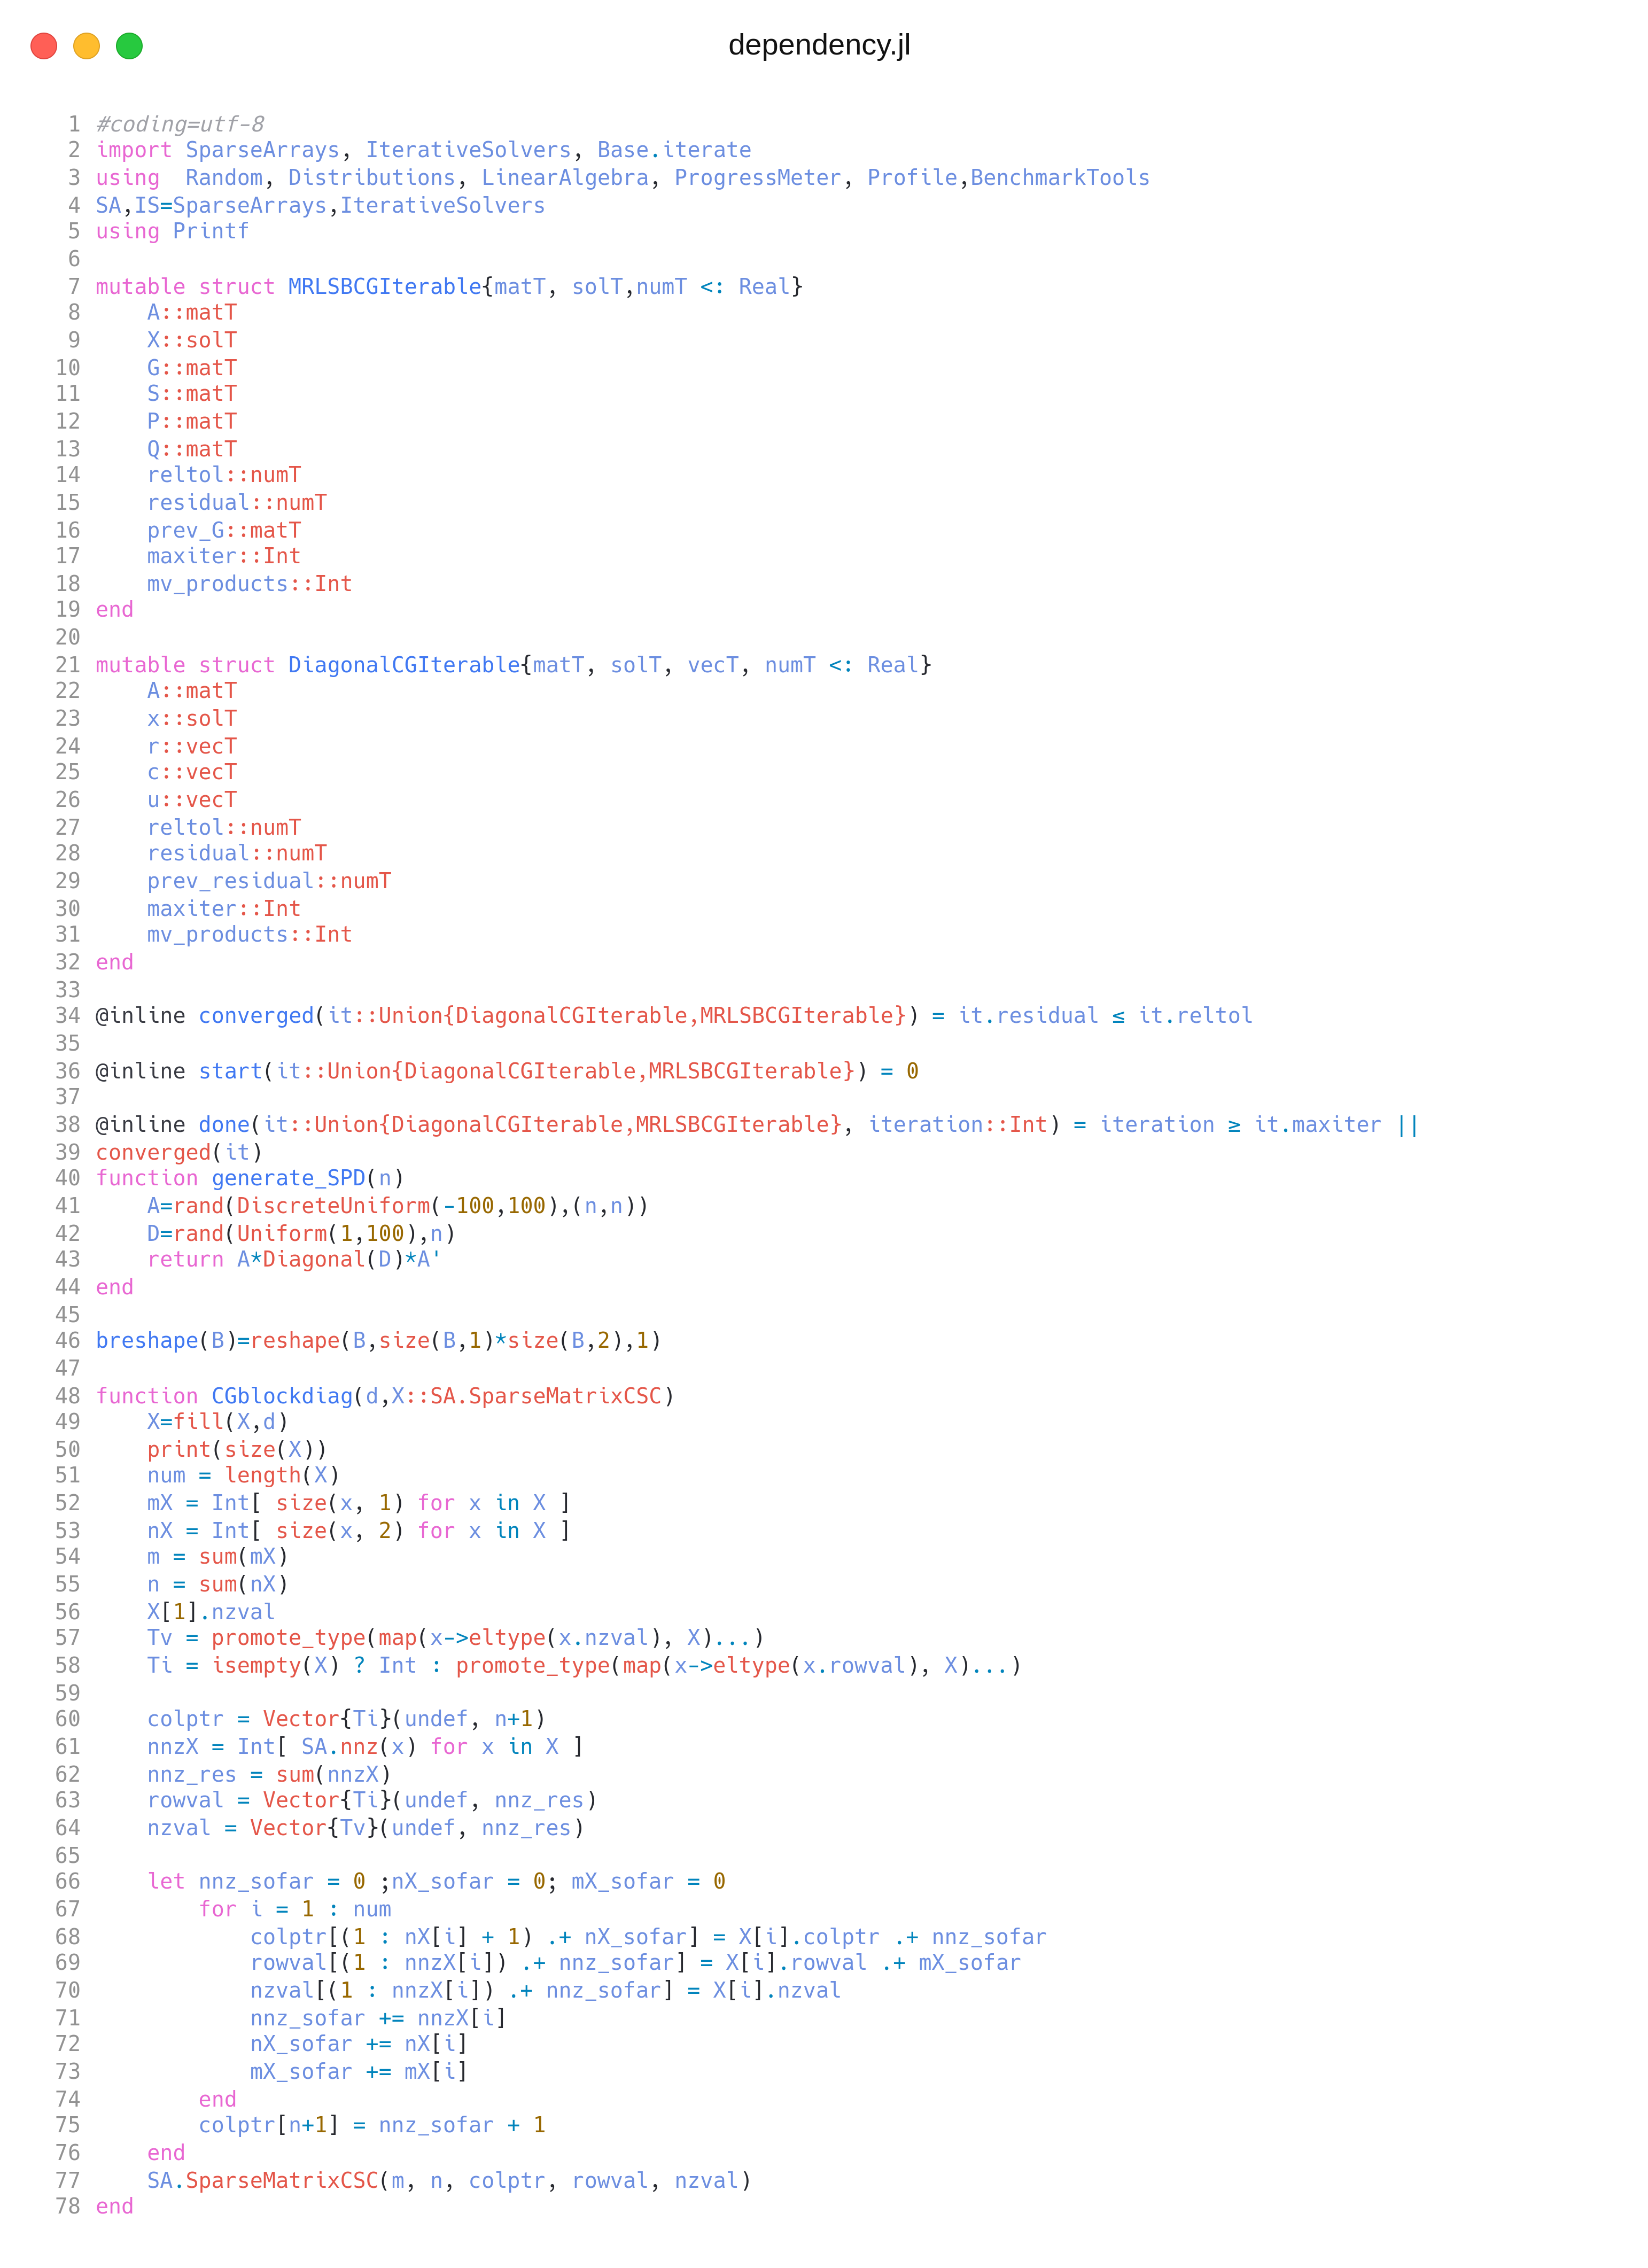
\includegraphics[height=0.9\textheight]{code/dependency.png}
 \end{figure}	    

\end {document}